
\section{Formal Definitions}
\label{sec:hublink_formal_definitions}

This section lays the formal foundation for the HubLink approach by providing definitions for the key concepts and data structures used throughout the approach. In the following, we first describe the underlying graph model to which the approach is applied. Then, we formally characterize the core elements specific to HubLink: \texttt{EntityWithDirection}, \texttt{HubRoot}, \texttt{HubPath}, \texttt{Hub}, and \texttt{HubVector}. These definitions are the prerequisites for the detailed algorithmic explanation in the following sections.

\subsection{Research Knowledge Graph (RKG)}

The underlying knowledge base is a \acrfull{rkg}, which is represented according to the \gls{rdf} standard \cite{wood_rdf_2014}. An \gls{rdf} graph provides a machine-readable semantic framework for describing ontologies, where information is expressed in the form of triples. The graph stores scholarly data where the triples capture not only bibliographic metadata (e.g., authors, dates, publishers) but also detailed relationships between scientific artifacts, for example, contributions of authors or publications. The formal definition of such an \gls{rdf} graph is provided in Section~\ref{sec:fundamentals_knowledge_graphs} and will not be repeated here.


\subsection{EntityWithDirection: Directed Graph Node}

An entity \( e \in E \) represents a node in the \gls{rdf} graph \( G \), where \( E \) is the set of all entities in the graph. Formally, the set of entities is defined as:
\[
E = \{ e \mid (s, p, o) \in G,\ e \in \{s, o\} \}.
\]

We define a path \( \mathcal{T} \) as a sequence of \( n \) triples, \( \mathcal{T} = [t_1, t_2, \ldots, t_n] \) where \( n \ge 1 \) and \( t_i = (s_i, p_i, o_i) \in G \) for all \( 1 \le i \le n \). This sequence represents a directed traversal through the graph \( G \), where adjacent triples are connected via shared entities.

When traversing such a path \( \mathcal{T} \), arriving at an entity \( e \) via the final triple \( t_n = (s_n, p_n, o_n) \) requires understanding the context: specifically, the path taken and whether \( e \) served as the subject or object. To capture this context, we introduce the \texttt{EntityWithDirection} structure. This structure associates an entity \( e \) with the specific path \( \mathcal{T} \) that ends at the entity, along with a direction indicator specifying the role of \( e \) in the final triple \( t_n \). 

Formally, we define an \texttt{EntityWithDirection} instance as a tuple \( (e, \text{dir}, \mathcal{T}) \). This tuple is constructed from a path \( \mathcal{T} = [t_1, \ldots, t_n] \), which terminates with the triple \( t_n = (s_n, p_n, o_n) \). The components \( e \) and \( \text{dir} \) are determined as follows:
\[
(e, \text{dir}) =
\begin{cases}
(s_n, \rightarrow) & \text{if the path reaches } s_n \text{ as the terminal entity} \\
(o_n, \leftarrow) & \text{if the path reaches } o_n \text{ as the terminal entity}
\end{cases}
\]
Here, \( \rightarrow \) indicates that the entity \( e \) is reached as the subject of the final triple, while \( \leftarrow \) signifies that the entity \( e \) is reached as the object.

We can now define the set \( \mathcal{D}_e \) for any given entity \( e \in E \), which includes all possible instances of \texttt{EntityWithDirection} instances that terminate at this specific entity \( e \):
\[
\mathcal{D}_e = \Big\{ (e, \text{dir}, \mathcal{T}) \;\Big|\;
\mathcal{T} = [t_1, \ldots, t_n], 
t_n = (s_n, p_n, o_n), 
(\text{dir} = \rightarrow \land e = s_n) \lor (\text{dir} = \leftarrow \land e = o_n)
\Big\}
\]

\subsection{HubRoot: Main Entity of a Hub}
\label{sec:hublink_hubroot_definition}

A \texttt{HubRoot} is an entity of the underlying \gls{rkg} and serves as the root entity of a hub. These are important for the construction of hubs, as each hub is built by collecting the paths starting from the root entity.

We denote the set of all \texttt{HubRoot} entities by \(R \subseteq V\), where \(V\) is the set of all entities in the graph \(G\). We formally define that the set of all hub roots is given by:
\[
R = \{\, v \in V \mid \phi(v) = 1 \,\},
\]
where $\phi(v)$ is a binary function to classify an entity as a \emph{HubRoot} if the criteria apply. Formally:
\[
\phi(v)=
\begin{cases}
1, & \text{if } v \text{ satisfies the hub root criteria}, \\
0, & \text{otherwise},
\end{cases}
\]

Whether \(v \in V\) is a member of \(R\) is determined by \(\phi(v)\). The criteria for defining hub roots can be based on various factors. In the following, we introduce some possibilities:

\begin{itemize}
    \item \textbf{Type-based:} The entity \(v\) has a specific type in \(G\). This is useful when the types of entities that are relevant for the \gls{qa} setting are known prior. For example, in the literature research setting, the objects of interest are publications. In this case, it is straightforward to define publications as hub types. 
    \item \textbf{Degree-based:} The degree of the outgoing edges of \(v\) exceeds a predefined threshold. This is useful when the information in a graph is highly diverse, making it difficult to define all possible types of hubs.
    \item \textbf{Path-based:} The number of paths at which \(v\) acts as the root where the paths reach a certain depth. 
    \item \textbf{Semantic-based:} The neighbors of \(v\) are checked for semantic similarity. If the similarity exceeds a predefined threshold, \(v\) is considered a root of the hub.
\end{itemize}

Defining the criteria for the hub roots is an ongoing process. We recommend choosing a hybrid approach from the methods suggested above and continually checking the coverage of the graph during indexing. It must be ensured that all entities relevant to the respective \gls{qa} setting are captured within a hub, as otherwise they cannot be fetched during the retrieval.


\subsection{HubPath: Path within a Hub}

A \texttt{HubPath} $h_r$ is built from the paths that start at a \texttt{HubRoot} $r \in R$ and lead to an end node. Each \texttt{HubPath} consists of a hash value, a textual description, and a list of \gls{rdf} triples. The hash value is used to uniquely identify the path and is generated by applying a hash function to the list of triples. The textual description is generated by an \gls{llm} and constitutes a natural language representation of $h_r$. The list of \gls{rdf} triples represents the path itself and is constructed by traversing the graph starting from the \texttt{HubRoot} entity, following the directed nature of the \gls{rdf} graph, to an end entity. 

Formally, let \(K \in \mathbb{N}\) be a predetermined maximum path length. The triple path of the \texttt{HubPath} $h_{r,i}$ is defined as a sequence
\[
\mathcal{T}_{h_{r,i}} = \langle t_1, t_2, \dots, t_k \rangle, \quad 1 \le k \le K,
\]
where each element \(t_j\) is an \gls{rdf} triple
\[
t_j = \bigl( v_{j-1}, p_j, v_j \bigr) \in G,
\]
with the convention that the initial entity \(v_0 = r\). In this context, \(v_{j-1}\) and \(v_j\) are entities, and \(p_j \in \mathcal{I}\) is the predicate. 

The following conditions are imposed on \(\mathcal{T}_{h_{r,i}}\):
\begin{enumerate}
  \item \textbf{Acyclic:} The set of entities \(\{v_0, v_1, \dots, v_k\}\) that are included in the path is required to be pairwise distinct. 
  \item \textbf{Single Outbound Degree:} Each intermediate entity \(v_j\) (for \(1 \le j < k\)) appears exactly once as the object of a triple and exactly once as the subject of a triple.
  \item \textbf{Termination:} The path terminates when at least one of the following conditions hold:
  \begin{enumerate}
    \item \emph{End of Graph:} The current entity \(v_k\) has no outgoing \gls{rdf} triple in \(G\).
    \item \emph{New Hub Root:} The current entity \(v_k\) is itself a hub root (i.e., \(v_k \in R\)).
    \item \emph{Maximum Length:} The path has reached the predetermined maximum length, \(k = K\).
  \end{enumerate}
\end{enumerate}

To preserve semantic continuity, it is important to monitor the length of the triple paths. If the paths are too long, the information from a hub might be too diverse and not semantically connected. If this is the case, reducing the maximum length of the paths can help. An alternative strategy is to adapt the definition of the \texttt{HubRoots}, which introduces more hubs and thus can also shorten the overall lengths of the \texttt{HubPaths}. However, if the paths are becoming too short, the information might not be detailed enough to answer a question. Therefore, it is important to monitor the lengths of the paths in the graph when building the index.

\begin{figure}[t]
    \centering
    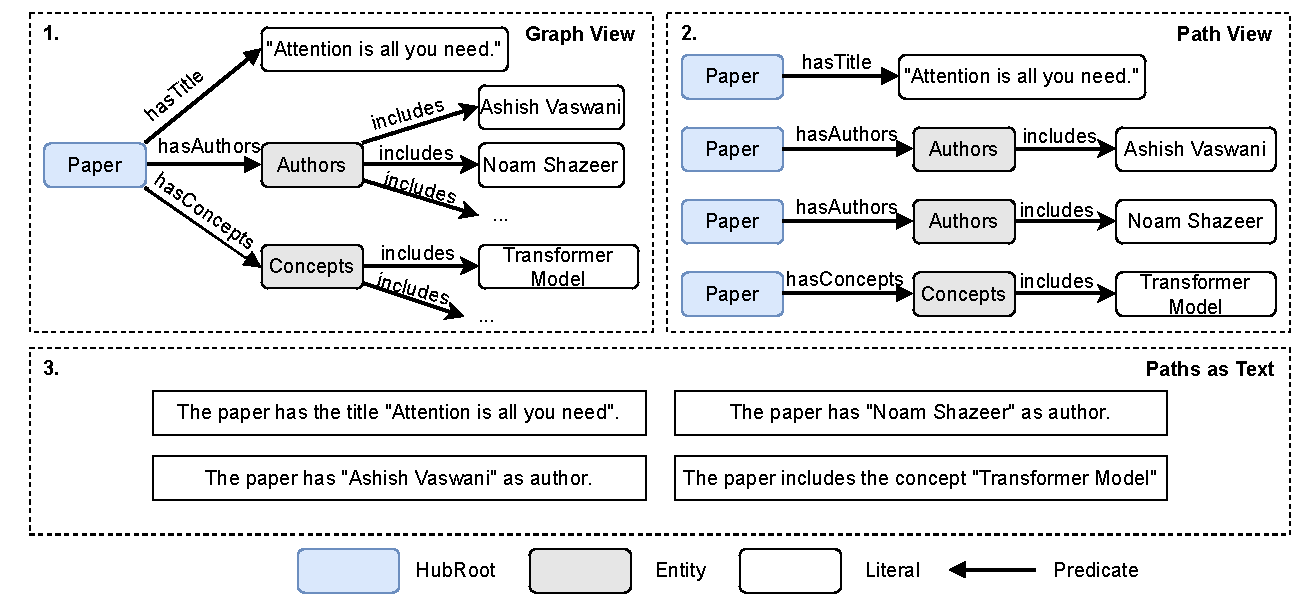
\includegraphics[width=1.0\linewidth]{figures/hublink/Hublink_figures-build_hubs.drawio.pdf}
    \caption[Path to Text Conversion]{Conversion of paths consisting of triples to textual descriptions using an \gls{llm}.}
    \label{fig:path_to_text_conversion}
\end{figure}

With the triple path $\mathcal{T}_{h_{r,i}}$, we can now define the hash value of the \texttt{HubPath} \(h_{r,i}\) as
\[
\phi_{r,i} = \text{hash}(\mathcal{T}_{h_{r,i}}) \in \mathcal{B},
\]
where \(\mathcal{B}\) is the set of all possible hash values. The hash value is generated by applying a hash function to the list of triples in the path. This will produce a unique value for each unique path, ensuring that no two paths have the same hash value, provided that the hash function is free from collisions. We then obtain the textual description of the \texttt{HubPath} \(h_{r,i}\) by applying a function:
\[
T_{\text{path}}: \mathcal{T}_{h_{r,i}} \to \mathcal{X},
\]
This function takes a triple path as input and outputs a textual description in a space \(\mathcal{X}\) of natural language strings. In \autoref{fig:path_to_text_conversion}, this process is illustrated. It shows the initial graph view and the decomposition of the hub subgraph into individual triple paths. These are then converted into a textual representation using the function \(T_{\text{path}}\) which is realized by an \gls{llm} that processes the sequence of \gls{rdf} triples $\mathcal{T}_{h_{r,i}}$ and generates a natural language description.

The final \texttt{HubPath} \(h_{r,i}\) is then defined as a tuple
\[
h_{r,i} = \bigl( \phi_{r,i}, T_{\text{path}}(\mathcal{T}_{h_{r,i}}), \mathcal{T}_{h_{r,i}} \bigr),
\]
where \(\phi_{r,i}\) is the hash value, \(T_{\text{path}}(\mathcal{T}_{h_{r,i}})\) is the textual description, and \(\mathcal{T}_{h_{r,i}}\) is the list of triples. The \texttt{HubPath} \(h_{r,i}\) is thus a representation of the path information inside a hub. This leads us to define the set of all \texttt{HubPaths} starting from the root of the hub \(r\). Formally, let \(r \in R\) be the root of the hub, where \(R\) is the set of \texttt{HubRoots} as defined in the previous section. 
We define the set of all HubPaths starting at \(r\) as
\[
\mathcal{H}(r) = \{\, h_r \mid h_r \text{ is a HubPath starting at } r \,\}.
\]

\subsection{Hub: Aggregation of Semantically Related Information}

A \texttt{Hub} is a special construct in the HubLink retriever that is used to aggregate semantically related information about a specific knowledge entity. It always consists of a \texttt{HubRoot} entity and a set of \texttt{HubPaths}. Formally, a hub is defined as
\[
Hub_r = \bigl( r,\, \mathcal{H}(r) \bigr),
\]
where \(r \in R\) is a hub root and \(\mathcal{H}(r)\) is the collection of hub paths starting from \(r\).

\subsection{HubVector: Encoding of Hub Information}
\label{sec:hublink_hubvector_definition}

To be able to efficiently retrieve relevant information from a hub, the \texttt{HubPaths} of the hub are encoded in a vector space using \texttt{HubVectors}. A \texttt{HubVector} is a low-dimensional vector representation constructed from the information of a \texttt{HubPath} and is always stored together with additional metadata that includes the hub root identifier \(r \in R\) and the textual description $T_{\text{path}}(\mathcal{T}_{h_{r,i}})$ of the \texttt{HubPath}. The goal is to project the semantic content of each \texttt{HubPath} into a vector space using a pre-trained embedding model, where a nearest-neighbor search such as \gls{ann} can be performed. What is important to consider here is that the path itself may contain too much information, which can lead to a phenomenon where the relevant information is obscured by the complexity of the path. To reduce this risk, the path is decomposed into different parts, increasing the likelihood of a nearest-neighbor search to find relevant information. More information on this design decision is provided in Section~\ref{sec:hublink_design_rationale}. 

By decomposing the \texttt{HubPath}, we define four vector representations. Let \(h_{r,i}\) denote the \(i\)-th \texttt{HubPath} of the hub with root \(r\). We define a general embedding function
\[
f: \mathcal{X} \to \mathbb{R}^d,
\]
which maps any textual input into a \(d\)-dimensional vector. We distinguish four types of \texttt{HubVectors} that can be generated from a hub path \(h_{r,i}\):

\begin{itemize}
    \item \textbf{Path Vector:} This vector represents the overall semantic content of the \texttt{HubPath}. It is obtained by embedding the full natural language description $T_{\text{path}}(\mathcal{T}_{h_{r,i}})$ of the path $\mathcal{T}_{h_{r,i}}$ generated by the \gls{llm}:
    \[
    \mathbf{v}_{\text{path}}(h_{r,i}) = f\Bigl( T_{\text{path}}(\mathcal{T}_{h_{r,i}}) \Bigr) \in \mathbb{R}^d
    \]
    
    \item \textbf{Triple Vector:} For this vector type, the triple path $\mathcal{T}_{h_{r,i}}$ is broken down into its individual triples. Each triple \(t_k \in \mathcal{T}_{h_{r,i}}\) is converted into a vector representation:
    \[
    \mathcal{V}_{\text{triples}} = \{f (t_k) \mid t_k \in \mathcal{T}_{h_{r,i}}\}, \quad f(t_k) \in \mathbb{R}^d
    \]
    
    \item \textbf{Entity Vector:} For this vector type, the triple path $\mathcal{T}_{h_{r,i}}$ is decomposed into all entities contained in the path. For each triple \(t_k = (s,p,o) \in \mathcal{T}_{h_{r,i}}\) , the entities \(s\) and \(o\) are extracted. Each entity is then embedded using \(f\):
    \[
    \mathcal{V}_{\text{entities}} = \{f(e) \mid t_k = (s, p, o) \in \mathcal{T}_{h_{r,i}},\ e \in \{s, o\}\}, \quad f(e) \in \mathbb{R}^d
    \]

    \item \textbf{Predicate Vector:} For this vector type, the hub path \(h_{r,i}\) is decomposed into all predicates contained in the path. For each triple \(t_k = (s,p,o) \in \mathcal{T}_{h_{r,i}}\), the predicate $p$ is extracted and embedded using \(f\). The embedding for each predicate is then computed as:
    \[
    \mathcal{V}_{\text{predicates}} = \{f(p) \mid t_k = (s, p, o) \in \mathcal{T}_{h_{r,i}}\}, \quad f(p) \in \mathbb{R}^d
    \]
\end{itemize}

For each hub path \(h_{r,i}\), multiple \texttt{HubVectors} are thus stored in the vector store. Each vector is stored as a tuple containing the root of the hub \(r\), the natural language description \(T_{\text{path}}(\mathcal{T}_{h_{r,i}})\), and the corresponding vector representation. Formally, we define the set of all \texttt{HubVectors} for \(h_{r,i}\) as:
\[
\begin{aligned}
    \mathcal{V}(h_{r,i}) =\;
    & \Bigl\{ \bigl( r,\; T_{\text{path}}(\mathcal{T}_{h_{r,i}}),\; \mathbf{v}_{\text{path}}(h_{r,i}) \bigr) \Bigr\} \\
    & \cup \Bigl\{ \bigl( r,\; T_{\text{path}}(\mathcal{T}_{h_{r,i}}),\; v \bigr) \mid v \in \mathcal{V}_{\text{triples}} \Bigr\} \\
    & \cup \Bigl\{ \bigl( r,\; T_{\text{path}}(\mathcal{T}_{h_{r,i}}),\; v \bigr) \mid v \in \mathcal{V}_{\text{entities}} \Bigr\} \\
    & \cup \Bigl\{ \bigl( r,\; T_{\text{path}}(\mathcal{T}_{h_{r,i}}),\; v \bigr) \mid v \in \mathcal{V}_{\text{predicates}} \Bigr\} \\
\end{aligned}
\]

Note that each vector is stored alongside the textual path description \(T_{\text{path}}(\mathcal{T}_{h_{r,i}})\) because decomposing the path into individual triples, entities, or predicates results in a loss of the semantic relationships between nodes. This can lead to reduced retrieval performance when a query matches a triple, entity, or predicate, as the isolated vector may not capture enough context to represent the full meaning. To address this, the textual description of the path \(T_{\text{path}}(\mathcal{T}_{h_{r,i}})\) is stored as metadata within each vector tuple. While the vector is used for similarity-based retrieval, the associated textual description is used during answer generation.

Finally, given a hub \(Hub_r = (r, \mathcal{H}(r))\), the overall set of \texttt{HubVectors} for the hub is defined as:
\[
\mathcal{V}(Hub_r) = \bigcup_{h \in \mathcal{H}(r)} \mathcal{V}(h).
\]
This collection of vectors, together with their associated metadata, forms the basis for the retrieval process in HubLink.
